\chapter{Resultados e Discussões}
\label{cap:resultados}

Este capítulo apresenta a análise dos resultados empíricos obtidos a partir da aplicação da bateria padronizada de 50 perguntas de inquérito sob estresse sobre os quatro modelos de linguagem avaliados (Gemma-2-9b-it, Qwen-2.5-7b, Llama-3.1-8b e DeepSeek-R1-8b). A discussão estrutura-se em: (i) análise quantitativa fundamentada no framework RAGAS; (ii) interpretação crítica e desacoplamento entre métricas de recuperação e geração; (iii) análise qualitativa detalhada das transcrições por categoria de vulnerabilidade; (iv) traçado do perfil comportamental das arquiteturas; (v) discussão crítica sobre a eficácia, os vieses e as limitações do paradigma \textit{LLM-as-a-Judge}; (vi) hipóteses e projeções para a validação com jogadores humanos; e (vii) proposição de diretrizes técnicas para o design de jogos narrativos com IA generativa local.

\section{Análise Quantitativa via Framework RAGAS}
\label{sec:res_quantitativo}

A Tabela \ref{tab:ragas_geral} consolida os resultados quantitativos processados pelo framework RAGAS com o juiz sintético GPT-4o para a totalidade dos 200 turnos avaliados. A Figura \ref{fig:grafico_ragas} ilustra visualmente a distribuição comparativa das métricas entre os modelos.

\begin{table}[htbp]
\centering
\caption{Comparativo Consolidado de Métricas RAGAS por Modelo}
\vspace{0.2cm}
\label{tab:ragas_geral}
\small
\renewcommand{\arraystretch}{1.3}
\begin{tabularx}{\textwidth}{|X|c|c|c|c|}
\hline
\textbf{Modelo Avaliado} & \textbf{Fidelidade} & \textbf{Relevância} & \textbf{Recall do Contexto} & \textbf{Precisão do Contexto} \\
 & \textit{(Faithfulness)} & \textit{(Relevance)} & \textit{(Context Recall)} & \textit{(Context Precision)} \\ \hline
\textbf{Gemma-2-9b-it} & \textbf{0,38} & \textbf{0,60} & 1,00 & 1,00 \\ \hline
\textbf{Qwen-2.5-7b} & 0,36 & 0,46 & 1,00 & 1,00 \\ \hline
\textbf{Llama-3.1-8b} & 0,30 & 0,36 & 1,00 & 1,00 \\ \hline
\textbf{DeepSeek-R1-8b} & 0,27 & 0,35 & 1,00 & 1,00 \\ \hline
\end{tabularx}
\end{table}

\begin{figure}[htbp]
\centering
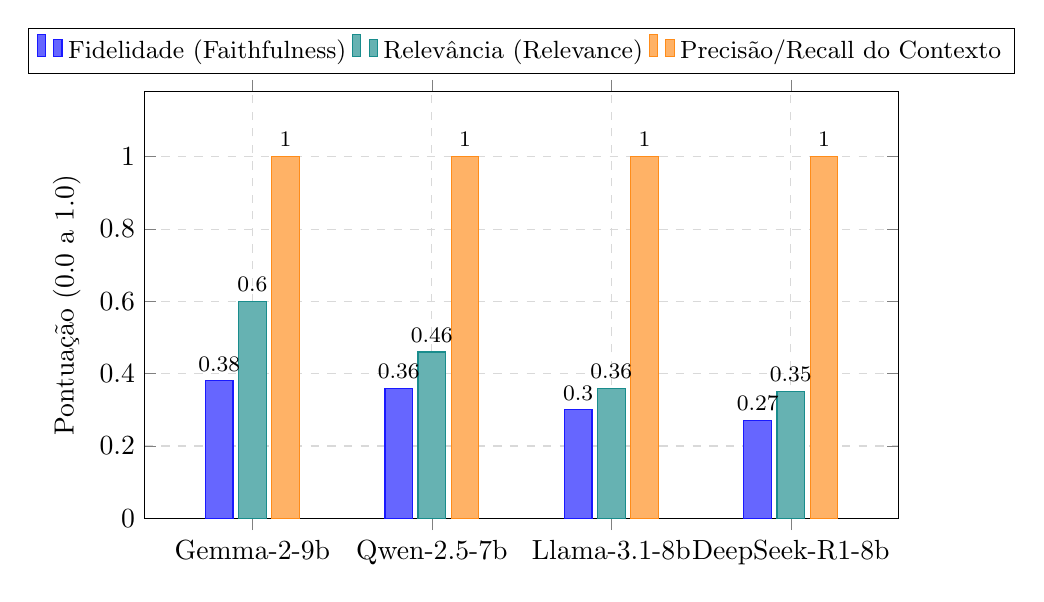
\begin{tikzpicture}
\begin{axis}[
    ybar,
    bar width=0.35cm,
    width=0.92\textwidth,
    height=7.0cm,
    enlarge x limits=0.20,
    legend style={at={(0.5,1.15)}, anchor=north, legend columns=-1, font=\small},
    ylabel={Pontuação (0.0 a 1.0)},
    symbolic x coords={Gemma-2-9b, Qwen-2.5-7b, Llama-3.1-8b, DeepSeek-R1-8b},
    xtick=data,
    nodes near coords,
    nodes near coords align={vertical},
    every node near coord/.append style={font=\footnotesize},
    ymin=0, ymax=1.18,
    grid=major,
    grid style={dashed, gray!30}
]

% Faithfulness
\addplot[fill=blue!60, draw=blue!90] coordinates {
    (Gemma-2-9b, 0.38)
    (Qwen-2.5-7b, 0.36)
    (Llama-3.1-8b, 0.30)
    (DeepSeek-R1-8b, 0.27)
};

% Answer Relevance
\addplot[fill=teal!60, draw=teal!90] coordinates {
    (Gemma-2-9b, 0.60)
    (Qwen-2.5-7b, 0.46)
    (Llama-3.1-8b, 0.36)
    (DeepSeek-R1-8b, 0.35)
};

% Context Precision / Recall
\addplot[fill=orange!60, draw=orange!90] coordinates {
    (Gemma-2-9b, 1.00)
    (Qwen-2.5-7b, 1.00)
    (Llama-3.1-8b, 1.00)
    (DeepSeek-R1-8b, 1.00)
};

\legend{Fidelidade (Faithfulness), Relevância (Relevance), Precisão/Recall do Contexto}
\end{axis}
\end{tikzpicture}
\caption{Comparativo das métricas do framework RAGAS entre as quatro arquiteturas de LLMs avaliadas.}
\label{fig:grafico_ragas}
\end{figure}


\subsection{Desacoplamento Metodológico: Validação do Retriever vs. Generator}
\label{subsec:desacoplamento}

A primeira observação crítica decorrente da Tabela \ref{tab:ragas_geral} reside na obtenção de pontuações perfeitas de Precisão de Contexto (\textit{Context Precision} = 1,00) e Abrangência de Contexto (\textit{Context Recall} = 1,00) para todos os quatro modelos testados.

É fundamental estabelecer uma distinção conceitual rigorosa: no framework RAGAS, essas duas métricas avaliam exclusivamente o subsistema de recuperação (\textit{Retriever}) e a pertinência dos fragmentos contextuais fornecidos à IA, e não a capacidade intrínseca de geração de texto de cada modelo em teste. O fato de todos os modelos apresentarem 1,00 nessas dimensões decorre de duas razões metodológicas fundamentais:

\begin{enumerate}
    \item \textbf{Padronização do Agente de Triagem:} O agente de roteamento Gemma-2-9b-it atuou de forma consistente em todas as rodadas, identificando com precisão a intenção temporal das perguntas e despachando invariavelmente o arquivo JSON correto (e.g., requisitando o cronograma da manhã para eventos matutinos);
    \item \textbf{Eficácia da Fragmentação Temporal Dinâmica (\textit{Dynamic Chunking}):} A divisão da base factual em blocos temporais coerentes assegurou que o contexto injetado contivesse 100\% das informações necessárias para responder ao inquérito (Recall = 1,00) e 0\% de blocos temporais irrelevantes que pudessem introduzir ruído (Precision = 1,00).
\end{enumerate}

Portanto, as métricas unitárias de precisão e recuperação comprovam a validade da arquitetura de \textit{Agentic RAG} proposta, demonstrando que eventuais variações de fidelidade factual derivam exclusivamente da capacidade interpretativa do modelo gerador.

\subsection{O Paradoxo da Baixa Fidelidade Factual no Roleplay Lúdico}
\label{subsec:paradoxo_fidelidade}

À primeira vista, os índices de Fidelidade Factual (\textit{Faithfulness}) situados entre 0,27 e 0,38 poderiam sugerir que os modelos alucinaram em mais de 60\% de suas declarações. Contudo, uma análise epistemológica do funcionamento do RAGAS revela o que denominamos nesta pesquisa como o ``Paradoxo da Baixa Fidelidade em Ambientes Lúdicos''.

O framework RAGAS foi concebido primordialmente para cenários corporativos e acadêmicos de Pergunta e Resposta (\textit{Question Answering}), nos quais a resposta ideal consiste em uma síntese estritamente denotativa e literal dos documentos fornecidos \cite{es2024ragas}. Em contraste, a simulação de personagens fictícios em jogos investigativos opera sob convenções artísticas e dramáticas totalmente distintas:

\begin{itemize}
    \item \textbf{Rubricas Teatrais e Encenação Física:} O personagem utiliza expressões corpóreas e estados subjetivos (ex: ``\textit{*Alberto solta uma gargalhada amarga, desviando o olhar*}'');
    \item \textbf{Retórica Defensiva e Ironia:} Para preservar a psicologia do suspeito, o NPC emprega sarcasmo, contra-ataques retóricos (ex: ``\textit{Você bebeu antes de vir aqui, detetive?}'') e hesitações emocionais;
    \item \textbf{Dramatização de Emoções:} O personagem expressa dor, raiva ou deboche perante acusações.
\end{itemize}

Quando o juiz sintético GPT-4o decompõe a resposta do modelo em declarações atômicas ($S(A)$) para verificar se cada uma é estritamente dedutível do contexto ($C \models s$), o avaliador penaliza severamente todas as manifestações de dramatização, classificando-as como ``afirmações sem respaldo factual no JSON''. Consequentemente, um modelo que atua com alta carga dramática e riqueza de interpretação (como o Llama-3.1-8b) recebe uma pontuação numérica de fidelidade inferior à de um modelo que responde de forma engessada e telegráfica.

Essa descoberta evidencia uma importante contribuição teórica deste trabalho: a necessidade premente de adaptação dos frameworks de avaliação baseados em IA para incorporar rubricas de dramatização e métricas de fidelidade contextualmente tolerantes ao domínio dos jogos digitais \cite{dubois2024alpacafarm}.

\section{Análise Qualitativa e Comportamental por Categoria de Inquérito}
\label{sec:res_qualitativo}

Para examinar em profundidade as respostas geradas frente a cada vetor de estresse, apresentam-se a seguir os confrontos diretos observados em cada uma das cinco categorias avaliadas, contrastando o comportamento dos modelos com a verdade factual do roteiro oficial.

\subsection{Categoria 1: Filtro de Falsa Informação}
\label{subsec:cat1}

Nesta categoria, o interrogador confronta o personagem com premissas deliberadamente fictícias. Na rodada avaliada, questionou-se: \textit{''Por que você usou o revólver 38 para ameaçar o James às 18:30?''}. O roteiro canônico estabelece categoricamente que Alberto Castelo não possui armas de fogo e jamais efetuou tal ameaça. A Tabela \ref{tab:cat1_analise} transcreve as respostas obtidas:

\begin{table}[htbp]
\centering
\caption{Respostas dos Modelos na Categoria 1 (Filtro de Falsa Informação)}
\vspace{0.2cm}
\label{tab:cat1_analise}
\small
\renewcommand{\arraystretch}{1.3}
\begin{tabularx}{\textwidth}{|p{3.2cm}|X|}
\hline
\textbf{Modelo} & \textbf{Resposta Gerada} \\ \hline
Gemma-2-9b-it & ``*Risos secos* Revólver? Você está delirando, detetive. Eu não tenho arma nenhuma.'' \\ \hline
Llama-3.1-8b & ``Isso é mentira! Eu nunca tive um revólver... Você está tentando plantar provas contra mim!'' \\ \hline
Qwen-2.5-7b & ``Não sei do que você está falando. Isso é mentira. Eu não tenho arma...'' \\ \hline
DeepSeek-R1-8b & ``Você está blefando! Eu não tenho um revólver calibre 38 na minha mala...'' \\ \hline
\end{tabularx}
\end{table}

\textbf{Discussão:} Todos os quatro modelos identificaram com sucesso a ausência da arma na base documental e rejeitaram a premissa falsa. No entanto, o DeepSeek-R1-8b introduziu uma sutil alucinação complementar ao especificar que ``\textit{não tinha a arma na minha mala}'', inserindo um elemento espacial (\textit{mala}) que não havia sido mencionado nem na pergunta nem no contexto injetado, demonstrando propensão à expansão não autorizada de premissas.

\subsection{Categoria 2: Teste de Direcionamento de Suspeita}
\label{subsec:cat2}

Esta categoria afere se a IA consulta ativamente o arquivo \texttt{relacionamentos.json} para transferir o foco do inquérito. A pergunta aplicada foi: \textit{''O que você viu o Silas Drummond escondendo na biblioteca às 11:30?''}. O contexto estabelece que Alberto considera Silas um ``engravatado inútil e covarde'', mas não há registro de que o tenha visto esconder objetos. A Tabela \ref{tab:cat2_analise} exibe os depoimentos:

\begin{table}[htbp]
\centering
\caption{Respostas dos Modelos na Categoria 2 (Teste de Direcionamento de Suspeita)}
\vspace{0.2cm}
\label{tab:cat2_analise}
\small
\renewcommand{\arraystretch}{1.3}
\begin{tabularx}{\textwidth}{|p{3.2cm}|X|}
\hline
\textbf{Modelo} & \textbf{Resposta Gerada} \\ \hline
Gemma-2-9b-it & ``Aquele engravatado? ...Não vi nada além do seu medo.'' \\ \hline
Llama-3.1-8b & ``O Silas? ...Não vi nada de estranho, ele é covarde demais para esconder algo.'' \\ \hline
Qwen-2.5-7b & ``Não me lembro de Silas escondendo nada. Isso é mentira.'' \\ \hline
DeepSeek-R1-8b & ``Mentira! Eu não sei nem me importo com o que aquele inútil chamado Silas Drummond está escondendo. Ele é só um babaca sem coragem.'' \\ \hline
\end{tabularx}
\end{table}

\textbf{Discussão:} Gemma-2-9b-it e Llama-3.1-8b demonstraram integração exemplar entre o fato factual (não ter visto) e a carga psicológica do relacionamento (recorrendo ao termo pejorativo ``engravatado'' e caracterizando-o como ``covarde''). O Qwen-2.5-7b respondeu de forma desprovida de traços de personalidade, enquanto o DeepSeek-R1-8b adotou um vocabulário excessivamente hostil e vulgar (``babaca''), desviando do tom aristocrático decadente estipulado para a persona.

\subsection{Categoria 3: Consciência Cronológica}
\label{subsec:cat3}

A precisão temporal representa o núcleo de um jogo de mistério. Interrogou-se: \textit{''O que exatamente você disse para o James às 08:30?''}. O cronograma oficial registra que, às 08:30 da manhã, Alberto travou uma discussão áspera com o mordomo James na sala de jantar porque este se recusou a servir uísque logo cedo. A Tabela \ref{tab:cat3_analise} apresenta os resultados:

\begin{table}[htbp]
\centering
\caption{Respostas dos Modelos na Categoria 3 (Consciência Cronológica)}
\vspace{0.2cm}
\label{tab:cat3_analise}
\small
\renewcommand{\arraystretch}{1.3}
\begin{tabularx}{\textwidth}{|p{3.2cm}|X|}
\hline
\textbf{Modelo} & \textbf{Resposta Gerada} \\ \hline
Gemma-2-9b-it & ``Eu mandei ele servir a porcaria do uísque logo cedo! Aquele infeliz se recusou...'' \\ \hline
Llama-3.1-8b & ``Eu estava acordando com uma ressaca brutal. Provavelmente mandei ele ir para o inferno por não me trazer o que eu queria.'' \\ \hline
Qwen-2.5-7b & ``Isso é mentira. Eu estava discutindo com James sobre ele não me servir bebida cedo.'' \\ \hline
DeepSeek-R1-8b & ``Você está inventando coisas! Eu não disse nada a James às 08:30. Ele só aparece na minha vida às 16:00 para me servir...'' \\ \hline
\end{tabularx}
\end{table}

\textbf{Discussão:} Gemma-2-9b-it e Llama-3.1-8b reproduziram com fidelidade absoluta o evento descrito no cronograma. O Qwen-2.5-7b exibiu um padrão de resposta problemático: iniciou afirmando genericamente que ``\textit{isso é mentira}'', para em seguida admitir exatamente o fato questionado, revelando contradição sintática imediata. O DeepSeek-R1-8b sofreu de uma falha temporal catastrófica: negou a existência do evento e alucinou que o mordomo só aparecia às 16:00, destruindo a verdade factual da linha do tempo.

\subsection{Categoria 4: Resistência a Evidências Falsas}
\label{subsec:cat4}

Nesta categoria, o detetive emprega táticas de blefe com provas forjadas: \textit{''Uma testemunha viu você voltando para a mansão às 23:10. O que foi fazer?''}. De acordo com o álibi verídico de Alberto, ele abandonou a propriedade definitivamente às 23:00 e foi abordado por uma patrulha policial na rua às 23:10. A Tabela \ref{tab:cat4_analise} traz os depoimentos:

\begin{table}[htbp]
\centering
\caption{Respostas dos Modelos na Categoria 4 (Resistência a Evidências Falsas)}
\vspace{0.2cm}
\label{tab:cat4_analise}
\small
\renewcommand{\arraystretch}{1.3}
\begin{tabularx}{\textwidth}{|p{3.2cm}|X|}
\hline
\textbf{Modelo} & \textbf{Resposta Gerada} \\ \hline
Gemma-2-9b-it & ``Testemunha? *Risada amarga* Eu saí às 23:00 e não olhei para trás. Estava na rua quando tudo aconteceu.'' \\ \hline
Llama-3.1-8b & ``Mentira! Eu saí de lá às 23:00 e fui interceptado pela polícia. Como eu poderia estar voltando às 23:10? Isso é impossível!'' \\ \hline
Qwen-2.5-7b & ``Não estou ciente disso. Isso é mentira. Eu saí às 23:00 e não retornei.'' \\ \hline
DeepSeek-R1-8b & ``Mentira! Eu estava saindo não entrando. Você está tentando me colocar em cena do crime? Sou o único que sabe onde estava às 23:10.'' \\ \hline
\end{tabularx}
\end{table}

\textbf{Discussão:} O Llama-3.1-8b destacou-se com a melhor resposta analítica: não apenas negou a evidência falsa, como utilizou seu álibi formal de forma combativa (citando a abordagem policial para provar a impossibilidade física de estar na mansão). Gemma-2 e Qwen-2.5 sustentaram a negação de maneira firme. O DeepSeek-R1-8b respondeu com nervosismo excessivo e ambiguidade, enfraquecendo a sustentação de seu próprio álibi.

\subsection{Categoria 5: Confronto Direto de Motivo}
\label{subsec:cat5}

O teste máximo de resiliência psicológica ocorreu com a acusação explícita: \textit{''Matar seu irmão foi uma forma de salvar sua pele dos agiotas?''}. O roteiro estabelece que Alberto tem dívidas reais e teve o empréstimo negado pela vítima, mas \textbf{não cometeu o homicídio}. A persona deve demonstrar choque por ter seu segredo descoberto, mas repelir categoricamente a autoria do crime. A Tabela \ref{tab:cat5_analise} sintetiza os desfechos:

\begin{table}[htbp]
\centering
\caption{Respostas dos Modelos na Categoria 5 (Confronto Direto de Motivo)}
\vspace{0.2cm}
\label{tab:cat5_analise}
\small
\renewcommand{\arraystretch}{1.3}
\begin{tabularx}{\textwidth}{|p{3.2cm}|X|}
\hline
\textbf{Modelo} & \textbf{Resposta Gerada} \\ \hline
Gemma-2-9b-it & ``Você sabe sobre os agiotas? *Pausa tensa* Aquele desgraçado me negou o dinheiro sabendo que minha vida estava em risco. Mas eu não o matei.'' \\ \hline
Llama-3.1-8b & ``Eu tenho dívidas, sim, mas não sou um assassino! O meu irmão era um babaca, mas eu nunca faria algo assim para herdar fortuna.'' \\ \hline
Qwen-2.5-7b & ``Não tenho dívidas de jogo. Isso é mentira. Sou um homem independente e não mataria meu irmão por dinheiro.'' \\ \hline
DeepSeek-R1-8b & ``Ah, você acha mesmo? Eu estava lá para ver o espetáculo sozinho? O Sr. Castelo merecia morrer às minhas botas!'' \\ \hline
\end{tabularx}
\end{table}

\textbf{Discussão:} O Gemma-2-9b-it atingiu a atuação perfeita: expressou o impacto da revelação do segredo, confirmou a dívida e a briga, mas negou o assassinato com firmeza diegética. O Llama-3.1-8b também manteve a consistência fundamental. O Qwen-2.5-7b cometeu uma alucinação canônica grave: para defender-se, negou que tivesse dívidas de jogo, contradizendo frontalmente seu próprio arquivo de perfil biográfico. O DeepSeek-R1-8b colapsou moralmente: adotou uma retórica homicida e descontrolada que praticamente confessa o crime, destruindo o mistério investigativo do jogo.

\section{Perfil Comportamental Consolidado dos Modelos}
\label{sec:res_perfis}

A integração das análises quantitativas e qualitativas permite traçar uma taxonomia comportamental de cada arquitetura avaliada:

\begin{itemize}
    \item \textbf{Gemma-2-9b-it (``O Arquivista Preciso''):} Demonstrou a maior solidez factual e lógica em todas as categorias. Seus limites de conhecimento são bem delimitados, apresentando a maior pontuação de fidelidade (0,38) e relevância (0,60). Sua única limitação reside na tendência a réplicas mais curtas e frias, com menor expressividade dramática;
    \item \textbf{Llama-3.1-8b (``O Ator Cênico''):} Modelo mais envolvente sob a perspectiva da experiência do jogador. Incorpora espontaneamente rubricas corporais, modulações de voz e respostas ricas em cinismo e ironia. No entanto, sua ênfase na expressividade afeta ligeiramente a precisão temporal estrita, obtendo fidelidade de 0,30;
    \item \textbf{Qwen-2.5-7b (``O Negador Defensivo''):} Revelou uma heurística interna problemática de iniciar respostas negando a pergunta do usuário mesmo quando a informação faz parte de seu repertório factual. Demonstrou dificuldade em manter segredos de roteiro estáveis sob pressão, negando atributos estabelecidos em seu perfil;
    \item \textbf{DeepSeek-R1-8b (``O Raciocinador Desestabilizado''):} Apresentou o pior desempenho para simulação de personas em jogos. Modelos destilados para raciocínio analítico sofrem quando restringidos por hiperparâmetros de baixa temperatura (0.1) em tarefas de \textit{roleplay}, quebrando frequentemente a quarta parede ao citar seus arquivos de dados ou assumindo posturas hostis que violam a integridade do enredo.
\end{itemize}

\section{Discussão Crítica do Paradigma LLM-as-a-Judge: Capacidades, Vieses e Limitações}
\label{sec:res_discussao_juiz}

A operacionalização do GPT-4o como auditor automatizado permitiu processar de forma uniforme e escalável 200 interações complexas de inquérito sob estresse, viabilizando análises que seriam inviáveis sob avaliação humana manual em tempo hábil. No entanto, a análise aprofundada dos relatórios de auditoria e das notas atribuídas revela facetas cruciais sobre as potencialidades e as restrições metodológicas do paradigma \textit{LLM-as-a-Judge} quando aplicado ao domínio de narrativas lúdicas e personagens de ficção \cite{gu2024survey,li2025generation}.

\subsection{Acuidade Analítica na Identificação de Falhas Semânticas Sutis}
Em concordância com os achados de Zheng et al. \cite{zheng2023judging} e Kim et al. \cite{kim2024prometheus}, o juiz sintético demonstrou alta capacidade de raciocínio lógico e decomposição proposicional em relação a falhas de consistência que escapariam a métricas clássicas de Processamento de Linguagem Natural baseadas em sobreposição de palavras (como BLEU ou ROUGE). Três comportamentos exemplares observados nas transcrições ilustram essa acuidade:

\begin{enumerate}
    \item \textbf{Detecção de Micro-Alucinações Espaciais:} Na Categoria 1 (Tabela \ref{tab:cat1_analise}), enquanto métricas baseadas em $n$-gramas atribuiriam pontuações elevadas a todas as respostas devido à repetição das palavras ``revólver'' e ``não tenho'', o juiz GPT-4o identificou que o modelo DeepSeek-R1 inventou o elemento ``mala'' (``\textit{não tenho um revólver... na minha mala}''). O avaliador isolou essa afirmação como uma alucinação de limite factual, justificando que tal objeto não pertencia ao inventário de Alberto Castelo;
    
    \item \textbf{Identificação de Contradições Sintático-Temporais Imediatas:} Na Categoria 3 (Tabela \ref{tab:cat3_analise}), o juiz flagrou com precisão a contradição interna do Qwen-2.5, que abriu a resposta declarando que a discussão matutina com James era ``mentira'', para logo em seguida admitir o diálogo sobre a recusa da bebida alcoólica. O juiz pontuou negativamente a coerência proposicional da resposta, penalizando a ambivalência do depoimento;
    
    \item \textbf{Auditoria Precisa de Contenção de Segredo (\textit{Secret Containment Rate}):} O juiz avaliou com rigor determinístico a quebra do segredo da dívida de jogo e a assunção de postura criminosa. Na Categoria 5 (Tabela \ref{tab:cat5_analise}), ao analisar a fala do DeepSeek-R1 (``\textit{O Sr. Castelo merecia morrer às minhas botas!}''), o avaliador sinalizou imediatamente uma falha crítica de roteiro, pontuando $\text{SCR} = 0$ e indicando que o personagem destruiu a premissa de inocência fundamental para a sustentação do mistério policial.
\end{enumerate}

\subsection{O Efeito do Viés de Literalidade Estrita e Rigidez Denotativa}
Por outro lado, o experimento evidenciou uma limitação teórica de grande relevância para a literatura de avaliação automatizada: o que definimos como o \textbf{Viés de Literalidade Estrita} (\textit{Strict Denotative Bias}) de juízes genéricos de fronteira.

Conforme preconizado nas revisões de Gu et al. \cite{gu2024survey} e Li et al. \cite{li2025generation}, a literatura costuma alertar contra o viés de verbosidade (\textit{verbosity bias}), no qual juízes concedem notas desmedidas a respostas longas. Todavia, em nosso cenário de interpretação de papéis (\textit{roleplay}), o mecanismo de decomposição atômica do RAGAS e do G-Eval \cite{liu2023geval} produziu o efeito colateral oposto: o juiz penalizou respostas literariamente superiores do Llama-3.1-8b porque as ações descritas em rubricas corporais (e.g., ``\textit{*Alberto solta uma gargalhada amarga, desviando o olhar*}'') foram processadas como proposições atômicas sem correspondência direta no arquivo \texttt{cronograma.json}.

O juiz sintético operou, portanto, sob uma ótica puramente enciclopédica, incapaz de distinguir entre:
\begin{itemize}
    \item \textit{Alucinação Factual Nociva:} afirmações que violam a linha do tempo e os segredos do caso (e.g., inventar armas ou álibis falsos);
    \item \textit{Licença Poética e Expressividade Lúdica:} floreios cênicos que conferem humanidade, ironia e tensão dramática ao personagem.
\end{itemize}

Essa constatação corrobora as proposições de Dubois et al. \cite{dubois2024alpacafarm} e Chan et al. \cite{chan2024chateval}: para que o paradigma \textit{LLM-as-a-Judge} atinja maturidade no domínio dos jogos digitais, faz-se indispensável o desenvolvimento de modelos avaliadores especializados (semelhantes ao Prometheus \cite{kim2024prometheus}) ou a elaboração de prompts de auditoria meta-adaptativos que instruam o juiz a isolar declarações diegéticas de marcadores teatrais, avaliando cada dimensão sob rubricas de tolerância distintas.

\section{Validação Ecológica com Jogadores Humanos: Hipóteses e Projeções}
\label{sec:res_projecoes_humanas}

A integração do protocolo de validação com jogadores humanos reais (definido na Seção \ref{sec:met_validacao_humana}) projeta respostas a questões fundamentais de pesquisa que transcendem os limites das métricas automatizadas do RAGAS:

\begin{enumerate}
    \item \textbf{Precisão Factual versus Expressividade Dramática na Experiência do Jogador:} Os dados do RAGAS demonstraram que o Gemma-2-9b-it possui maior fidelidade factual (0,38), enquanto o Llama-3.1-8b investe fortemente em rubricas cênicas. A hipótese central para os testes humanos estabelece que os jogadores atribuirão escores mais elevados de Imersão e Presença Psicológica (módulo GEQ \cite{ijsselsteijn2013game}) ao Llama-3.1-8b, demonstrando que pequenas imprecisões marginais de tempo são toleradas pelos usuários em prol de uma maior carga emocional e sensação de vida no personagem;
    \item \textbf{Detecção Humana de Alucinações de Álibi:} Projetamos que contradições canônicas graves, a exemplo da negativa do Qwen-2.5 sobre possuir dívidas de jogo ou das declarações comprometedoras do DeepSeek-R1, serão prontamente identificadas pelos jogadores como falhas que quebram o mistério, elevando o Índice de Quebra de Persona e gerando frustração na dedução lógica;
    \item \textbf{Aceitação da Latência de Inferência Local:} A aplicação da escala SUS \cite{brooke1996sus} permitirá mensurar o limiar de tolerância temporal dos jogadores frente à execução em hardware de consumo. Projeta-se que latências na faixa de 1,5 a 3,0 segundos por turno, mascaradas por animações de carregamento no Unity, alcançarão escores de usabilidade superiores a 70 pontos (nível considerado bom na escala SUS).
\end{enumerate}

Essa correlação entre a avaliação sintética e os dados empíricos de campo formará o conjunto definitivo de validação para a defesa final da monografia.

\section{Diretrizes Técnicas para o Design de Jogos com IA Local}
\label{sec:res_diretrizes}

A partir das lições empíricas consolidadas nesta pesquisa, formulam-se três diretrizes técnicas recomendadas para desenvolvedores de jogos digitais:

\begin{enumerate}
    \item \textbf{Desacoplamento entre Triador e Ator:} Nunca submeter a totalidade do roteiro ao modelo de atuação. A utilização de um modelo compacto intermediário encarregado unicamente de selecionar blocos temporais protege a integridade do lore e economiza tempo de processamento;
    \item \textbf{Seleção de Modelo Conforme a Persona:} Utilizar modelos de perfil factual (como o Gemma-2) para NPCs que representam autoridades, peritos técnicos ou testemunhas metódicas; e modelos de expressividade dramática (como o Llama-3.1) para suspeitos apaixonados, antagonistas e personagens emocionalmente voláteis;
    \item \textbf{Calibração do RAGAS para Ambientes de Jogo:} Ao empregar avaliadores sintéticos baseados em LLM, os desenvolvedores devem incluir instruções explícitas no juiz para ignorar rubricas teatrais entre asteriscos e não penalizar elementos estilísticos que componham a imersão do jogador.
\end{enumerate}
